\begin{itemize}
	\item Input: An array $A$ of n integers and a rank $i$, with $1\ge i\ge n$.
	\item output: The element $x\in A$ that is larger than exactly $i-1$ other
	elements of $A$.
\end{itemize}
We can solve the selection problem in $O(n\log n)$ time since we
can sort the number using heapsort or mergesort and then simply index
the $i$-th element in the output array. But we can do better than this.

\subsection{Randomized-Select}
\begin{algorithm}[H]
	\SetKwProg{Fn}{Function}{:}{}
	\SetKwFunction{FRandSelect}{RANDOMIZED-SELECT}
	\SetKwFunction{FRandPartition}{RANDOMIZED-PARTITION}
	
	\Fn{\FRandSelect ($A, p, r, i$)}{
		%         \KwData{Array $A[p, \cdots, r]$, rank $i$}
		\uIf{p == r}{
			return A[p]
		}
		q = \FRandPartition(A, p, r){}
		
		k = q - p + 1 
		
		\uIf {i == k}{\tcc{The pivot is the answer}
			return A[q]
		}
		\uElseIf {i < k}{
			return \FRandSelect ($A, p, q-1, i$)
		}
		\Else{
			return \FRandSelect ($A, q+1, r, i-k$)
		}
		
	}
	\caption{Randomized-Select}
\end{algorithm}
The worst-case running time for RANDOMIZED-SELECT is $\Theta(n^2)$, because we 
could be extremely unlucky and always partition around the largest remaining 
element, and the partition takes $\Theta(n)$ times.

But the algorithm has a linear expected running time $O(n)$, and because it is 
randomized, no particular input elicits the worst-case behavior.

\subsection{Deterministic Linear Time Selection}
After quick selection, algorists looked for an algorithm which is able to solve 
the problem in linear deterministic.

\centerline{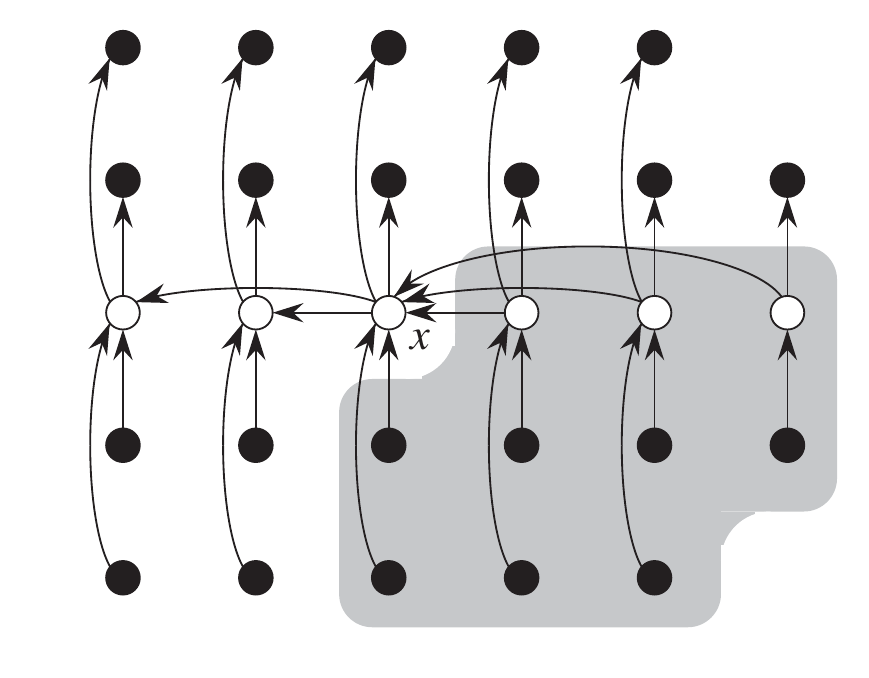
\includegraphics[width=0.5\textwidth]{deterministic-select.png}}
Given an array with $n$ numbers, we can find the element with rank $i$ by the following method.
	
SELECT Algorithm:
\begin{itemize}
	\item Partition the numbers into groups of size 5.
	\item Find the medium of each group. It can be done within 6 comparisons. $T(n) = \frac{6n}{5} 
	= 1.2n$.
	\item Use SELECT to recursively find the medium of the mediums $m^*$.
	\item $m^*$ has a rank somewhere in the middle.
	We treat the median of the medians $m^*$ as a pivot element and compare it with all elements to get its rank $k$, which takes $n$ steps.
	\begin{itemize}
		\item The number of elements larger than $m^*$: $O(\frac{3n}{10}) 
		=3(\ceil*{\frac{1}{2}\ceil*{\frac{n}{5}}})$
		\item Therefore, the number of element smaller than $m^*$: 
		$O(\frac{7n}{10})$.
	\end{itemize}
	\item Pivot using $m^*$:
	\begin{itemize}
		\item If $i = k$, then return $k$.
		\item If $i < k$, use SELECT recursively to find the $i$-th smallest 
		element on the low side.
		\item If $i > k$, use SELECT recursively to find the $(i-k)$-th smallest 
		element on the high side.
	\end{itemize}
\end{itemize}
Therefore, the recursion of the algorithm is
\[T(n) \le T(\frac{n}{5}) + T(\frac{7n}{10}) + 2.2n\]
The expression does not fit into the master theorem frame work because of the 
two different size of the sub-problems. Then we guess $T(n) \le 22n$ and it can 
be proved by induction.
\begin{itemize}
	\item Base case:
	
	Base case it trivial and we skip it during the class because 22 is a 
	fairly large number. It should be easy find a number $n$ so that we could 
	calculate $T(n)$ easily and show that it is less than $22n$.
	
	\item Hypothesis: Suppose each of the cost satisfies $T(n) \le 22n$ for $(0, 
	n)$. 
	
	Therefore, 
	\begin{align*}
	T(\frac{n}{5}) &\le 22 \times \frac{n}{5}\\
	T(\frac{7n}{10}) &\le 22 \times \frac{7n}{10}\\
	\intertext{so that}
	T(n) &\le 22 \times 0.2 n + 22 \times 0.7 n + 2.2n
	\end{align*}
	\item Inductive step:
	\begin{align*}
	T(n) &\le 22 \times 0.2 n + 22 \times 0.7 n + 2.2n\\
	T(n) &\le 22 \times (0.2 + 0.7 + 0.1)n\\
	T(n) &\le 22n
	\end{align*}
\end{itemize}

\subsection{Efficiently Find Median in a Small Gorup}
The following algorithm gives pretty good upper bounds for finding the median for a small number of elements, although they are not the best upper bounds
for n > 6.

Suppose we are trying to find the $t$-th largest element of n,
\begin{itemize}
	
	\item Choose $n - t + 2$ of the elements arbitrarily, and find the largest one by tennis tournament like procedure. 
	
	\item Replace the largest element by one of the elements that hasn't yet participated in the tournament and make it play the same opponents that the largest element played to determine the new largest. r
	
	\item We keep doing this until all the elements that were set aside initially have played in the tournament. 
	
	\item We replace the largest element of the last round too (and hence are left with n - t + 1 elements).
	
	\item Now the largest element that remains is the one we are looking for.
\end{itemize}

\subsubsection{Correctness}
There are at most $(t-2)$ numbers larger than the largest element in the $(n - t + 2)$ element, say $x$. Every $x$ is the one of the top $t-1$ numbers. We repeat the tournament $t-1$ times to find all the top $t-1$ numbers. Then the largest one in the rest of $n - t + 1$ numbers has the rank $t$.

\subsubsection{Time}
\begin{itemize}
	\item The first tournament takes $(n - t + 1)$ comparisons. 
	\item Then the next $t - 2$ tournament only take $\log_2 (n - t + 2)$ times. \item Finally, find the one with rank $t$ takes one more tournament among $(\log_2 n - t + 2)$ elements.
\end{itemize}

\[T(n) = (n - t + 1) + (t -2 )\log_2 (n - t + 2) + \log_2 (n - t + 2)\]


